
\begin{table}[!ht]
\centering
\resizebox{\columnwidth}{!}{\begin{tabular}{|c|c|c|c|} 
\hline
Food & Vitamin A & Vitamin B & Cost \\
\hline
P & 3 units/kg & 5 units/kg & 60 Rs/kg \\ 
\hline
Q & 4 units/kg & 2 units/kg & 80 Rs/kg \\ 
\hline
Requirement & 8 units/kg & 11 units/kg & \\ 
\hline
\end{tabular}}
\caption{Food Requirements}
\label{opt/12/tab:table1}
\end{table}
Let the mixture contain $x$ kg of food P and $y$ kg of food Q be $y$  such that 
\begin{align}
    x \geq 0 \\
    y \geq 0 
\end{align}
According to the question,
\begin{align}
    3x+4y &\geq 8 \\
    5x+2y &\geq 11
\end{align}
$\therefore$ Our problem is
\begin{align}
        \min_{\vec{x}} Z &= \myvec{60 & 80}\vec{x}\\
        s.t. \quad 
        \myvec{3 & 4 \\ 5 & 2 }\vec{x} &\preceq \myvec{8\\11} \\
        \vec{x} &\preceq \vec{0}
\end{align}
Lagrangian function is given by
\begin{equation}
\begin{aligned}
    &L(\vec{x},\boldsymbol{\lambda}) \\ &= \myvec{60 & 80}\vec{x}+\lcbrak{\sbrak{\myvec{3 & 4}\vec{x}-8}} \\ &+ \sbrak{\myvec{5 & 2}\vec{x}-11} \\ &+ \sbrak{\myvec{-1 & 0}\vec{x}} +\rcbrak{\sbrak{\myvec{0 & -1}\vec{x}}}\boldsymbol{\lambda}
\end{aligned}
\end{equation}
where,
\begin{align}
    \boldsymbol{\lambda} &= \myvec{\lambda_1 \\ \lambda_2 \\ \lambda_3 \\ \lambda_4}
\end{align}
Now,
\begin{align}
    \nabla L(\vec{x},\boldsymbol{\lambda}) &= \myvec{60+ \myvec{3 & 5 & -1 & 0 }\boldsymbol{\lambda}\\ 80+\myvec{4 & 2 & 0 & -1}\boldsymbol{\lambda} \\ \myvec{3 & 4}\vec{x}-8 \\ \myvec{5 & 2}\vec{x}-11 \\ \myvec{-1 & 0}\vec{x} \\ \myvec{0 & -1}\vec{x}}
\end{align}
$\therefore$ Lagrangian matrix is given by
\begin{align}
    \myvec{0 & 0 & 3 & 5 & -1 & 0 \\ 0 & 0 & 4 & 2 & 0 & -1 \\ 3 & 4 & 0 & 0 & 0 & 0 \\ 5 & 2 & 0 & 0 & 0 & 0 \\ -1 & 0 & 0 & 0 & 0 & 0 \\ 0 & -1 & 0 & 0 & 0 & 0}\myvec{\vec{x} \\ \boldsymbol{\lambda} } &= \myvec{-60 \\ -80 \\ 8 \\ 11 \\ 0 \\0 }
\end{align}
Considering $\lambda_1,\lambda_2$ as only active multiplier,
\begin{align}
    \myvec{0 & 0 & 3 & 5 \\ 0 & 0 & 4 & 2 \\ 3 & 4 & 0 & 0 \\ 5 & 2 & 0 & 0}\myvec{\vec{x}\\ \boldsymbol{\lambda}} &= \myvec{-60 \\ -80 \\ 8 \\ 11}
\end{align}
resulting in,
\begin{align}
    \myvec{\vec{x} \\ \boldsymbol{\lambda}} &= \myvec{0 & 0 & 3 & 5 \\ 0 & 0 & 4 & 2 \\ 3 & 4 & 0 & 0 \\ 5 & 2 & 0 & 0}^{-1}\myvec{-60 \\-80 \\ 8 \\ 11}
    \\
    \implies   \myvec{\vec{x} \\ \boldsymbol{\lambda}} &= \myvec{0 & 0 & \frac{-28}{196} & \frac{56}{196} \\ 0 & 0 & \frac{70}{196} & \frac{-42}{196} \\ \frac{-28}{196} & \frac{70}{196} & 0 & 0 \\ \frac{56}{196} & \frac{-42}{196} & 0 & 0}\myvec{-60 \\-80 \\ 8 \\ 11}
    \\
    \implies \myvec{\vec{x} \\ \boldsymbol{\lambda}} &= \myvec{2 \\ \frac{1}{2} \\ -20 \\ 0 }
\end{align}
$\because \boldsymbol{\lambda}=\myvec{-20 \\ 0} \preceq \vec{0} $
\\
$\therefore$ Optimal solution is given by
\begin{align}
    \vec{x} &= \myvec{2\\ \frac{1}{2}} \\
    Z &= \myvec{60 & 80}\vec{x} \\
    &= \myvec{60 & 80}\myvec{2 \\ \frac{1}{2}} \\
    &= 160
\end{align}
By using cvxpy in python,
\begin{align}
    \vec{x}=\myvec{2.11436237\\0.41422822}\\
    Z = 159.99999999
\end{align}
Fig. \ref{opt/12/fig:Graphical Solution}	verifies this result.
%
\begin{figure}[!ht]
\centering
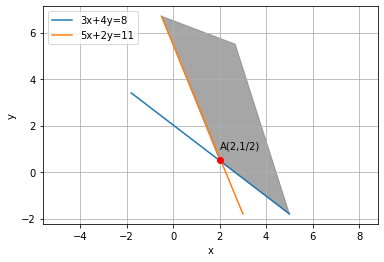
\includegraphics[width=\columnwidth]{solutions/su2021/2/12/Graphical Solution_10.png}
\caption{Graphical Solution}
\label{opt/12/fig:Graphical Solution}	
\end{figure}


